\chapter{Extending a Brainiac Prover to Higher-Order Logic}
\setheader{Extending a Brainiac Prover to Higher-Order Logic}
\label{ch:ehoh2}

% \renewcommand{chapter}[0]{chapter}
\newcommand\ehohii{$\lambda$E}


\authors{Joint work with\\
Jasmin~Blanchette and Stephan~Schulz}


\blfootnote{In this work I designed, implemented, and evaluated all changes to
term representation, algorithms, and indexing data structures. Jasmin Blanchette
did the daily supervision. Stephan Schulz provided
the necessary E expertise.}

\begin{abstract}%
    The automatic discharge of tedious subgoals is high on the wishlist of many
  users of proof assistants. Some proof assistants discharge such goals
  by translating them to first-order logic and invoking an efficient prover on
  them, but much is lost in translation. As an alternative,
  we propose to extend first-order provers with native support for
  higher-order features. Building on our extension of E to $\lambda$-free
  higher-order logic, we now extend E to full higher-order logic.
  The resulting prover is the \NumberOK{strongest} one on benchmarks coming from a
  proof assistant, and the \NumberOK{second strongest} on TPTP benchmarks.
    %It also incurs no overhead on first-order problems.  -- sounds like a detail --JB
\end{abstract}

\newpage

\section{Introduction and Background}
\label{sec:ehoh2:introduction}

In Chapter~\ref{ch:ehoh} of this thesis we introduced Ehoh, a rather conservative extension of
state-of-the-art first-order prover to a fragment of higher-order logic devoid of $\lambda$-abstraction. This
extension gave us a flavor of the difficulties that we might encounter on the
way to full higher-order logic. In chapters that precede this one,
we discussed many ways in which those difficulties can be overcome.
In this chapter, we fulfill a promise we gave in the beginning of the thesis: We present the extension of
Ehoh to full higher-order logic using incomplete variants
of $\lambda$-superposition. We call this prover \ehohii.

%
The $\lambda$-superposition calculi were
previously implemented in Zipperposition, and
extensive experiments with various heuristic choices have been performed
(Chapter \ref{ch:ho-techniques}). In \ehohii{}'s implementation, we used
these experiences to choose a set of effective rules that could easily be
retrofitted into an originally first-order prover. Another principle that guided 
the design of \ehohii{} was \emph{gracefulness}: We made sure that our changes
do not impact the strong first-order performance of E and $\lambda$-free higher-order performance of Ehoh. 

% We
% also used the experience of fine-tuning the calculi
% \cite{section-making-ho-work} in Zipperposition to carefully choose which
% calculus extensions and heuristics to use in E.

One of the main challenges we faced was retrofitting $\lambda$-terms in Ehoh's
term representation (Sect.~\ref{sec:ehoh2:terms}). Furthermore, Ehoh's main inference
engine was designed with the assumption that it will be used with
inferences that compute an MGU. We
implemented a higher-order unification procedure (Chapter \ref{ch:unif})
that can return multiple unifiers (Sect.~\ref{sec:ehoh2:unif-match-index}) and
integrated it in the inference engine. Finally, we extended and adapted the
rules of superposition calculus, resulting in an incomplete, pragmatic variant of
$\lambda$-superposition (Sect.~\ref{sec:ehoh2:calculus}).

We \NumberOK{evaluated} \ehohii{} on a selection of proof assistants benchmarks
as well as all higher-order theorems in the TPTP library \cite{gs-17-tptp}
(Sect.~\ref{sec:ehoh2:eval}). We found
that \ehohii{} clearly outperformed Ehoh on all benchmarks. It outperformed all other higher-order provers on the
proof assistant benchmarks; on the TPTP benchmarks it ended up second only 
to the cooperative version of Zipperposition, which employs Ehoh as a
backend. An arguably fairer comparison without the backend puts \ehohii{} in
first place for both benchmark suites.
We also compared the performance of \ehohii{} with E on first-order
%%% @PETAR: I made this slightly sentence shorter and more forceful. Please
%%% check if you agree. --JB
problems and found that little overhead has been introduced by the
extension to higher-order logic.

\ourpara{Background} The logic \ehohii{} targets is the monomorphic higher-order
logic described in Sect.~\ref{sec:pre:hol}. We reuse all the notions from this
section, with the corresponding notations. Like in the previous chapter, we
simplify the notation by writing predicate literals in unencoded form: Positive
literal $\eqlit{s}{\itrue}$ is written as $s$ and negative literal
$\neqlit{s}{\top}$ is written as $\negpredlit{s}$.   This chapter discusses
three tightly related provers E, Ehoh, and \ehohii{}, which are disambiguated as
follows:

\begin{itemize}
  \item E is a state-of-the-art first-order prover based on superposition. It is described in
  Sect.~\ref{sec:pre:theorem-provers}.
  \item Ehoh is an extension of E to support $\lambda$-free higher-order logic. Chapter \ref{ch:ehoh}
  is dedicated to Ehoh.
  \item \ehohii{} further builds on Ehoh to support full higher-order logic. It is the latest prover
  described in this chapter.
\end{itemize}

\section{Terms}
\label{sec:ehoh2:terms}

\looseness=-1
E has been designed around perfect term sharing %or exa
\cite{ls-01-shared}, a design that we carried on to  Ehoh and \ehohii{}: Any two structurally identical terms are
guaranteed to be the same object in memory. This is achieved through term
\emph{cells}, which represent individual terms. Each cell has (among other fields)
(1)~\texttt{f\_code}, an integer corresponding to the symbol at the head of the term (negative
if the head is a free variable, positive otherwise); (2)~\texttt{num\_args},
corresponding to the number of arguments applied to the head; and (3)~\texttt{args},
a size-\texttt{num\_args} array of pointers to argument terms. We
use the first-order notation $\cst{f}(s_1, \ldots, s_n)$ to denote a cell whose
\texttt{f\_code} corresponds to $\cst{f}$, \texttt{num\_args} equals $n$, and
\texttt{args} points to the cells for $s_1, \ldots s_n$.

Ehoh represents $\lambda$-free higher-order terms using flattened, spine notation
(Sect.~\ref{sec:ehoh:types-and-terms}).
Thus, the terms $\cst{f}$, $\cst{f} \, \cst{a}$, and $\cst{f} \, \cst{a} \,
\cst{b}$ are represented by the cells $\cst{f}$,
$\cst{f}(\cst{a})$, and $\cst{f}(\cst{a}, \cst{b})$, respectively.
To ensure free variables are
perfectly shared, Ehoh treats applied free variables differently: Arguments are
not applied directly to a free variable, but using an internal symbol
\internalat{} of variable arity. For example, the term $X \, \cst{a} \, \cst{b}$ is
represented by the cell $\internalat(X, \cst{a}, \cst{b})$. This ensures that
two different occurrences of the free variable $X$ correspond to the same object,
which makes substitutions more efficient.
%%% @PETAR(read): This tries to explain an invisible problem. Either we need to explain
%%% it better, or we just omit it (my favorite option). It's old Ehoh stuff anyway. --JB
%Yet, to
%efficiently access variable arguments we do not use binary application symbol,
%but flattened representation.

\ourpara{Representation of $\lambdabf$-Terms} To support full
higher-order logic, Ehoh's $\lambda$-free cell data structure must
be extended to support the $\lambda$ binder. We use the locally nameless
representation \cite{ac-12-locally-nameless} for this purpose: De Bruijn indices
%%% @PETAR(checked): Double-check "possibly loose".
represent (possibly loose) bound variables, whereas we keep the current
representation for free (and applied) variables.

%%% @PETAR(read): Sounds odd---we wouldn't be extending the term representation of an
%%% already HO prover. --JB
%Unlike other higher-order provers, most of which are written in functional
%programming languages,
Extending the term representation of Ehoh with a new term
kind involves intricate manipulation of the cell data structure. De Bruijn
indices must be represented as other cells with either a negative or a positive
\texttt{f\_code}. However, this has to be done in such a way that a De Bruijn
index can never be mistaken for a function symbol or a variable.

Other than possibly being instantiated during $\beta$-reduction, De Bruijn
indices mostly behave as constants. Therefore, we decided to represent De
Bruijn indices using positive \texttt{f\_code}s: The De Bruijn index of value $i$
will have $i$ as the~\verb|f_code|. To ensure De Bruijn indices are not
mistaken for function symbols, we use the \texttt{properties} bitfield of the
cell, which holds precomputed properties of %shared cell
%%% @PETAR(checked, you are right): I don't understand why you wrote "shared cell". Please double-check. --JB
the cell. We introduce the
property \texttt{IsDBVar} to denote that the cell represents a De
Bruijn index. Any attempt to create a De Bruijn index is performed through
a dedicated library function that sets the \texttt{IsDBVar} property for every term it
returns. When given the same De Bruijn index and type, this function is
guaranteed to always return the same object. Finally, we have guarded all the
functions and macros that manipulate function codes with the check if the
property \texttt{IsDBVar} is set. To ensure perfect sharing of every occurrence
of De Bruijn indices, arguments to De Bruijn indices are applied like for free
variables, using \internalat{}.

Extending cells to support $\lambda$-abstraction is easier. Each
$\lambda$-ab\-strac\-tion has the distinguished function code \internallam{} as the head
symbol and two arguments:\ (1)~a De Bruijn index 0 of the type of the abstracted variable;
(2)~the body %(matrix)
of the $\lambda$-abstraction. Consider
the term $\lambda x. \, \lambda y.\, \cst{f}\, x \, x$, where both $x$ and $y$ have
the type~$\iota$. This term is represented as $\lambda\,\lambda\, \cst{f} \,
\db{1} \, \db{1}$ in locally nameless representation, where bold numbers
represent De Bruijn indices. In \ehohii{}, the same term is represented by the cell
$\internallam(\db{0}, \internallam(\db{0}, \cst{f}(\db{1}, \db{1})))$,
where all De Bruijn variables have type~$\iota$. 

The first argument of $\internallam$ is
redundant, since it can be deduced from the type of the $\lambda$-abstraction.
However, basic $\lambda$-term manipulation operations often require access to
this term. We store it explicitly to avoid creating it repeatedly.

\ourpara{Efficient $\betabf$-Reduction}
Terms are stored in $\beta\eta$-reduced form. As these two reductions are
performed very often, they ought to be efficient. \ehohii{}
performs $\beta$-reduction by reducing the leftmost outermost $\beta$-redex
first. To represent $\beta$-redexes, it uses the \internalat{} symbol. Thus,
the term $(\lambda
x.\, \lambda y.\,  (x \, y)) \, \cst{f} \, \cst{a}$ is represented by
$\internalat(\internallam(\db{0}, \internallam(\db{0}, \internalat(\db{1}, \db{0}))),
\cst{f}, \cst{a})$. Another option would have been to add arguments applied to
$\lambda$-term directly to the $\lambda$ representation (as in
$\internallam(\db{0}, \internallam(\db{0}, \allowbreak \internalat(\db{1}, \db{0})),
\cst{f}, \cst{a})$), but this would break the invariant
that $\internallam$ has two arguments. Furthermore, replacing free
variables with $\lambda$-abstractions (e.g., replacing $X$ with $\lambda
x. \, x$ in $\internalat(X, \cst{a})$) would require additional normalization.

A term can be $\beta$-reduced as follows: When a cell of the
form $ \internalat(\internallam(\db{0}, s),t)$ is encountered, the field
\texttt{binding} (normally used to record the substitution for a free variable) of the
cell $\db{0}$ is set to $t$. Then $s$ is traversed to instantiate every
loose occurrence of $\db{0}$ in $s$ with \texttt{binding}, whose loose
bound De Bruijn indices are shifted by the number of $\lambda$ binders above
the occurrence of $\db{0}$ in $s$ \cite{fk-01-deBruijn}. Next, the same
procedure is performed on the resulting term and its subterms, in
leftmost outermost fashion.

\ehohii{}'s basic $\beta$-normalization mechanism works in this way, but it
features a few optimizations.
First, \ehohii{} recognizes terms of the form $(\lam{\overline{x}_n}{s}) \,\overline{t}_n$ 
and performs parallel replacement of the bound variables $x_i$ with
$t_i$. Since intermediate terms are not constructed, this reduces the number of
recursive function calls and calls to the cell allocator.

Second, in line with the gracefulness principle, we want \ehohii{} to incur
little (if any) overhead on first-order problems and to
excel on higher-order problems with a large first-order component. If
$\beta$-reduction is implemented naively, finding a $\beta$-redex involves
traversing the entire term. On purely first-order terms, $\beta$-reduction
is then a complete waste of time.

To avoid this, we use Ehoh's perfectly shared
terms and their \texttt{properties} field.
%
We introduce the property \texttt{HasBetaReducibleSubterm}, which is set if
%%% @PETAR(is is good): "is" or "may be" below? (Overapproximation?) --JB
a cell is $\beta$-reducible.
Whenever a new cell that contains a
$\beta$-reducible term as a direct subterm is shared, the property is set.
Setting of the property is inductively continued when further superterms are
shared. For example, in the term $t = \cst{f} \, \cst{a} \, (\cst{g} ((\lambda x.\,
x)\,\cst{a}))$, the cells for $(\lambda x.\, x)\,\cst{a}$,
$\cst{g}\,((\lambda x.\, x)\,\cst{a})$, and $t$ itself have the property
\texttt{HasBetaReducibleSubterm} set.
%
When it needs to find $\beta$-reducible subterms, \ehohii{} will visit only the
cells with this property set. This further means that on first-order
subterms, a single bit masking operation is enough to determine that no subterm
should be visited.

Along similar lines, we added a property \texttt{HasDBSubterm} that
caches whether the cell contains a De Bruijn subterm. This
%% @PETAR(you are right): Why "also"? What's the other thing?
%also
makes
instantiating De Bruijn indices during $\beta$-norma\-lization faster, since only the
subterms that contain De Bruijn indices must be visited. Similarly, some other
operations such as shifting De Bruijn indices or determining whether a term is closed
(i.e., it contains no loose bound variables) can be sped up or even avoided
if the term is first-order.

\ourpara{Efficient $\etabf$-Reduction}
The term $\lambda x.\, s \, x$ is $\eta$-reduced to $s$ whenever $x$ is not a loose bound variable
in $s$. Caching the property of $\eta$-reducibility of the term is not
as beneficial as the one for $\beta$-reducibility, because checking this
property at the term's top level is done in $O(|s|)$, compared with constant time
for $\beta$-reducibility.
However, we use the observation that a term cannot be $\eta$-reduced if it has
no $\lambda$-abstraction subterms and introduce a property \texttt{HasLambda}
that notes the presence of $\lambda$-abstraction in a term. Only
terms with this property are visited during $\eta$-reduction.

\ehohii{} performs parallel $\eta$-reduction: It recognizes terms of the form
$\lam{\overline{x}_n}{s \, \overline{x}_n } $ such that none of the $x_i$
occurs loose bound in $s$. If done naively, reducing terms of this kind requires up to $n$
traversals of $s$ to check if each $x_i$ occurs in $s$. In \ehohii{}, exactly one
traversal of $s$ is required.

\looseness=-1
More specifically, when $\eta$-reducing a cell $\internallam(\db{0}, s)$,
\ehohii{} considers all $\lambda$ binders in $s$ as well. In general,
the cell will be of the form
$\internallam(\db{0}, \dotsc,\allowbreak \internallam(\db{0}, t) \ldots)$,
where $t$ is not a
$\lambda$-abstraction, and $l$ is the number of $\internallam$ symbols above $t$. Then \ehohii{} breaks down the body~$t$ into a maximal
decomposition $u\, (\dbvar{n}\db{{}-1}) \, \ldots \, \db{1} \, \db{0}$.
If $n = 0$, the cell is not $\eta$-reducible.
Otherwise, $u$ is traversed to determine the
minimal index~$\dbvar{j}$ of a loose De Bruijn index,
taking $\dbvar{j} = \infty$ if no such index exists.
%%% @PETAR(I prefer leftmost as we are going top level left-to-right and not
%bottom-up as innermost can suggest): Check "innermost".
%%% @PETAR(you are right, but I will add righmost outermost to be more precise): But it's rightmost then not leftmost! In the example, the very first
%%% binder remains (the one to which the 2's point). --JB
We can then remove the $k = \min\{j,l,n\}$ rightmost outermost $\lambda$ binders in $\internallam(\db{0},
\ldots, \internallam(\db{0}, t) \ldots)$ and replace %the body
$t$ by the variant of
$u \allowbreak\, (\dbvar{n}\db{{}-1}) \allowbreak\, \ldots \, (\dbvar{k}\db{{}+1}) \, \dbvar{k}$
obtained by shifting the loose De Bruijn indices down by~$k$.

To better understand this convoluted De Bruijn arithmetic, consider the
term $\lambda x. \, \lambda y. \, \lambda z.\,\allowbreak \cst{f} \, x \, x \, y
\, z$. This term is represented by the cell $\internallam(\db{0},
\internallam(\db{0}, \internallam(\db{0},\allowbreak \cst{f}(\db{2}, \db{2}, \db{1},
\db{0}))))$. \ehohii{} splits $\cst{f}(\db{2}, \db{2}, \db{1}, \db{0})$ into
two parts:\ $u = \cst{f} \, \db{2}$ and the arguments $\db{2}, \db{1},
\db{0}$. Since the minimal index in $u$ is $\db{2}$, we can
omit the De Bruijn indices $\db{1}$ and $\db{0}$ and their $\lambda$ binders,
yielding the $\eta$-reduced cell $\internallam(\db{0}, \cst{f}(\db{0},
\db{0}))$.

The use of the \texttt{HasLambda} property ensures that $\eta$-reduction is not
tried on first-order or $\lambda$-free higher-order terms, whereas parallel
$\eta$-reduction both speeds up $\eta$-reduction and avoids creating a linear
number of intermediate terms. For finding the minimal loose De Bruijn index,
optimizations such as the \texttt{HasDBSub\-term} property are used.

\ourpara{Representation of Boolean Terms}
E represents Boolean terms using
term cells whose \texttt{f\_code}s correspond to internal codes reserved
for logical symbols. Quantified formulas are represented by cells in which the
first argument is the quantified variable and the second one is the body of the
quantified formula. For example, the term $\iforall x.\, \cst{p} \, x$ corresponds
to the cell $\iforall(X, \cst{p}(X))$, where $X$ is a regular free variable.
% as Ehoh has no concept of a bound variable.

This representation is convenient for parsing formulas and clausification, which
is what E uses it for, but it
causes $\alpha$-normalization issues during the actual proof search: In
full higher-order logic, Boolean terms can appear as subterms in clauses, as in
$\cst{q}(X) \llor \cst{p}(\iforall(X, \cst{r}(X)))$;
instantiating $X$ in the first literal should not influence $X$ in the second
literal.

To avoid this issue, in \ehohii{} we use $\lambda$ binders to represent quantified formulas.
Thus, $\iforall x. \, s$ is represented by $\iforall \, (\lambda x. \, s)$.
Quantifiers are then unary symbols that do not directly bind
the variables but delegate this responsibility to a $\lambda$-abstraction.
%
Since \ehohii{} represents bound variables using De Bruijn indices, this solves the
$\alpha$-conversion issues. However, this solution is incompatible with
thousands of decades-old lines of clausification code that assumes the E
representation of
quantified formulas. Therefore, \ehohii{} converts quantified
formulas only after clausification, for Boolean terms that appear in a
higher-order context (e.g., as argument to a function symbol).

\ourpara{New Term Orders}
The $\lambda$-superposition calculus is parameterized by a term order that is
used to break symmetries in the search space.
We implemented the versions of the Knuth--Bendix order (KBO) and lexicographic
path order (LPO) for higher-order terms with $\lambda$-abstractions described by
Bentkamp et al.~\cite{bbtv-21-full-ho-sup}. These orders
encode $\lambda$-terms as first-order terms and then invoke the standard KBO or
LPO. %Trading elegance for efficiency, our
%implementation does not compute the first-order translation.
%Rather,
For efficiency, we implemented separate KBO and
LPO functions that compute the order directly, intertwining the encoding and
the order computation.
%%% @PETAR(yes): Irrelevant detail?
%We kept the
%implementation of $\lambda$-free KBO as \ehohii{} can be run in $\lambda$-free mode.

Ehoh cells contain a \verb|binding| field that can be used to store the
substitution for a free variable. Substitutions can then be applied by following
the \texttt{binding} pointers, replacing each free variable with its instance.
Thus, when Ehoh needs to perform a KBO or LPO comparison of an instantiated term,
it needs only follow the \texttt{binding} pointers.
In full higher-order logic, however, instantiating a variable can trigger a
series of $\beta\eta$-reductions,
changing the shape of the term dramatically. To prevent this, \ehohii{}
computes the $\beta\eta$-reduced instances of the terms
before comparing them using KBO or LPO.

\section{Unification, Matching, and Term Indexing}
\label{sec:ehoh2:unif-match-index}


Standard superposition crucially depends on the concept of an MGU. In higher-order logic, such a unifier does not in general exist,
and the concept
%%% @PETAR: CSU, infinite
is replaced by that of a complete set of unifiers (CSU), which may be infinite.
In Chapter \ref{ch:unif}, we described an efficient procedure to enumerate a CSU
for a term pair. It is implemented in Zipperposition, together with some
extensions to term indexing. In \ehohii{}, we further improve the performance of
this procedure by implementing a terminating, incomplete variant. We also
introduce a new indexing data structure.

\subsection{The Unification Procedure} 
% Two main guiding principles behind our
% unification procedure are laziness and redundancy elimination. The first one is
% embodied in the fact that the procedure makes sure that it never fully
% normalizes the terms or fully applies the substitution if that is not necessary.
% Redundancy elimination is achieved through \emph{oracles}
% \cite{unif-section}: the procedures that solve the unification
% problem for a subclass of higher-order terms on which unification is decidable,
% and for \ehohii{}, unary. If those procedures determine that the given terms
% belong to their class of terms, they will return the most general unifier,
% avoiding redundant computations and in some cases even non-termination.
The unification procedure works by maintaining a list of unification pairs to be solved.
After choosing a pair, it first normalizes it by $\beta$-reducing and
instantiating the heads of both terms in the pair. Then, if either head is a
variable, it computes an appropriate binding for this variable, thereby
approximating the solution.

Unlike in first-order and $\lambda$-free higher-order unification, in the full
higher-order case there may be many bindings that lead to a solution. To reduce
this mostly blind guessing of bindings, the procedure features support for
\emph{oracles} (Sect.~\ref{sec:unif:the-unification-procedure}). These are
procedures that solve the unification problem for a subclass of higher-order
terms on which unification is decidable and, in the case of \ehohii{}, unary. Oracles help
increase performance, avoid nontermination, and avoid redundant bindings.

\looseness=-1
In Chapter \ref{ch:unif}, the unification procedure is described as a transition system. In
\ehohii{}, the procedure is implemented nonrecursively, and the unifiers are
enumerated using an iterator object that encapsulates the unifier
search state. The iterator consists of five fields:
\begin{enumerate}
  \item \vn{constraints}, which holds the unification
  constraints
  \item \vn{bt\_state}, a stack that contains information necessary to backtrack
  to a previous state
  \item \vn{branch\_iter}, which stores how far we
  are in exploring different possibilities from the current search node
  \item \vn{steps}, which remembers how many different unification bindings (such as
  imitation, projection, and identification) are applied
  \item \vn{subst},
  a stack storing the variables bound so far
\end{enumerate}
\pagebreak[2]
\newcommand{\cn}[1]{\ensuremath{\textsc{#1}}} %const name
\newcommand{\fc}[1]{\ensuremath{\textsc{#1}}} %function call
\algrenewcommand\alglinenumber[1]{{\color{gray} \tiny #1}}

The iterator is initialized to hold the original problem in \vn{constraints},
and all other fields are initially empty. The unifiers are retrieved one by one by
calling the function \fc{ForwardIter}. It returns \fc{True} if the iterator made
progress, in which case the unifier can be read via the iterator's
$\vn{subst}$ field. Otherwise, no more unifiers can be found, and the iterator is
no longer valid. The function's pseudocode is given below, including two
auxiliary functions \fc{NormalizeHead} and \fc{BacktrackIter}:

\vspace{\jot}
\begin{algorithmic}[]
  \Function{ForwardIter}{$\vn{iter}$}
  \State $\vn{forward} \gets \neg \vn{iter.constraints.empty()} \lor \fc{BacktrackIter}(\vn{iter})$
  \While{$\vn{forward} \land \neg \vn{iter.constraints.empty()}$}
    \State $(\vn{lhs}, \vn{rhs}) \gets $ pop pair from $\vn{iter.constraints}$
    \State $\vn{lhs} \gets \fc{NormalizeHead}(\vn{lhs})$
    \State $\vn{rhs} \gets \fc{NormalizeHead}(\vn{rhs})$
    \State normalize and discard the $\lambda$ prefixes of $\vn{lhs}$ and $\vn{rhs}$

    \If{$\neg\vn{lhs.head.is\_var()} \land \vn{rhs.head.is\_var()}$}
      \State swap $\vn{lhs}$ and $\vn{rhs}$
    \EndIf

    \If{$\vn{lhs.head.is\_var()}$}
      \State $\vn{oracle\_res} \gets \fc{Fixpoint}(\vn{lhs, rhs, iter.subst}) $
      \If{$\vn{oracle\_res} = \cn{NotInFragment}$}
        \State $\vn{oracle\_res} \gets \fc{Pattern}(\vn{lhs, rhs, iter.subst}) $
      \EndIf

      \If{$\vn{oracle\_res} = \cn{NotUnifiable}$}
        \State $\vn{forward} \gets \fc{BacktrackIter(iter)}$
      \ElsIf{$\vn{oracle\_res} = \cn{NotInFragment}$}
        \State $\vn{n\_steps}, \vn{n\_branch\_iter}, \vn{n\_binding} \gets$
        \State $\quad \fc{NextBinding}(\vn{lhs}, \vn{rhs}, \vn{iter.steps}, \vn{iter.branch\_iter})$
        
        \If{$\vn{n\_branch\_iter} \not= \fc{BindEnd}$ }
          \State push pair $(\vn{lhs},\vn{rhs})$ back to \vn{iter.constraints}
          \State push quadruple $(\vn{iter.constraints}, \vn{n\_branch\_iter}, $
          \State                  $\quad \vn{iter.steps}, \vn{iter.subst})$ onto $\vn{iter.bt\_state}$
          \State extend $\vn{iter.subst}$ with $\vn{n\_binding}$
          \State $\vn{iter.steps} \gets \vn{n\_steps}$
          \State $\vn{iter.branch\_iter} \gets \cn{BindBegin}$
        \ElsIf{\vn{lhs.head = rhs.head}}
          \State push the constraint pairs of arguments of $\vn{lhs}$ and $\vn{rhs}$
                 to \vn{iter.constraints}
          \State $\vn{iter.branch\_iter} \gets \cn{BindBegin}$
        \EndIf
      \EndIf
    \ElsIf{$\vn{lhs.head} = \vn{rhs.head}$}
    \State push the constraint pairs of arguments of $\vn{lhs}$ and $\vn{rhs}$
           to \vn{iter.constraints}
    \Else{} \State $\vn{forward} \gets \fc{BacktrackIter(\vn{iter})}$
    \EndIf
  \EndWhile
  \State \Return $\vn{forward}$
  \EndFunction
  \vspace{2\jot}
  \pagebreak[2]
  
  \Function{NormalizeHead}{$\vn{t}$}
    \If{$\vn{t.head} = \internalat \land \vn{t.args}[0].\vn{is\_lambda}()$}
      \State reduce the top-level $\beta$-redex in $t$
      \State \Return $\fc{NormalizeHead}(t)$
    \ElsIf{$\vn{t.head.is\_var()} \land \vn{t.head.binding} \not= \cn{nil}$}
      \State $\vn{t.head} \gets \vn{t.head.binding}$
      \State \Return $\fc{NormalizeHead}(t)$
    \Else{}
      \State \Return $t$
    \EndIf
  \EndFunction
  
  \vspace{\jot}
  \Function{BacktrackIter}{$\vn{iter}$}
    \If{\vn{iter.bt\_state.empty()}}
      \State clear all fields in \vn{iter}
      \State \Return \cn{False}
    \Else
    \State pop $(\vn{constraints}, \vn{branch\_iter}, \vn{steps}, \vn{subst})$ from $\vn{iter.bt\_state}$
    \State set the corresponding fields of $\vn{iter}$
    \State \Return \cn{True}
    \EndIf
  \EndFunction
  \vspace{\jot}
  
\end{algorithmic} 

\looseness=-1
\fc{ForwardIter} begins by backtracking if the previous attempt was successful (i.e., 
all constraints were solved). If it finds a state from which it can continue,
it takes term pairs from $\vn{constraints}$ until
there are no more constraints or it is determined that no unifier exists. The terms
are normalized by instantiating the head variable with its binding and then
reducing the potential top-level $\beta$-redex that appears. This instantiation
and reduction process is repeated
until there are no more top-level $\beta$-redexes and the head is
not a variable bound to some term. Then the term with shorter
$\lambda$ prefix is expanded (only on the top level) so that $\lambda$ prefixes have the
same length. Finally, the $\lambda$ prefix is ignored, and we
focus only on the body. In this way, we avoid fully substituting
and normalizing terms and perform just enough operations
to determine the next step of the procedure.

If either term of the constraint is flex, we first invoke oracles to solve the
constraint. \ehohii{} implements the most efficient oracles implemented in
Zipperposition:\ fixpoint and pattern (Sect.~\ref{sec:unif:implementation}). An oracle can return three results:
(1)~there is an MGU for the pair (\cn{Unifiable}), which is recorded in
\emph{subst}, and the next pair in $\emph{constraints}$ is tried;
(2)~no MGU exists
for the pair (\cn{NotUnifiable}), which causes the iterator to backtrack;
% to previous state;
(3)~if the pairs do not belong to the subclass that oracle
can solve (\cn{NotInFragment}), we generate possible variable bindings---that is,
we guess the approximate form of the solution.

\ehohii{} has a special module that generates bindings (\cn{NextBinding}). This
module is given the current constraint and the values of \emph{branch\_iter} and
\emph{steps}, and it either returns the next binding and the new values of
\emph{branch\_iter} and \emph{steps} or reports that all different variable
bindings are exhausted. The bindings that \ehohii{}'s unification procedure creates
are imitation, Huet-style projection, identification, and elimination (one
argument at a time) (Sect.~\ref{sec:unif:the-unification-procedure}). A limit on the
total number of applied binding rules can be set, as well as a limit on the
number of individual rule applications. The binding module checks whether limits
are reached using the iterator's \vn{steps} field.

Computing bindings is the only point in the procedure where the search tree
branches and different possibilities are explored. Thus, when \ehohii{} follows
the branch indicated by the binding module, it records the state to which it
needs to return, should the followed branch be backtracked. The state consists of
the values
of $\vn{constraints}, \vn{steps}$, and $\vn{subst}$ before the branch is followed
and the value of \vn{branch\_iter} that points past the followed branch. The
values of \vn{branch\_iter} are either \cn{BindBegin}, which denotes that no
binding was created, intermediate values that \cn{NextBinding} uses to remember
how far through bindings it is, and \cn{BindEnd}, which indicates that all
bindings are exhausted.

If all bindings are exhausted, the procedure checks whether the pair is
flex--flex and both sides have the same head. If so, the pair is decomposed and
constraints are derived from the arguments of the pair. Otherwise, the iterator
backtracks.
% @PETAR(actually the procedure applies bindings to same-head flex-flex pairs,
% so the text is OK -- we do get "stuck" enumerating those flex-flex pairs. The
% limits help here): Maybe explain here that you don't want a pragmatic prover
% like lambdaE to get stuck in wildly explosive flex-flex pairs? --JB
%
If the constraint is rigid--rigid, for unification to succeed, the heads of both
sides of the constraint must be the same. Unification then continues
with new constraints derived from the arguments. Otherwise, the iterator must be
backtracked.

\subsection{Matching} 

In E, the matching algorithm is mostly used inside
simplification rules such as demodulation and subsumption \cite{ss-02-brainiac}.
As these rules must be efficiently performed, using any complex matching
algorithm is not a viable option. Instead, we implemented a matching algorithm
for the pattern class of terms \cite{tn-93-patterns} to complement Ehoh's
$\lambda$-free higher-order matching algorithm (Sect.~\ref{sec:ehoh:unif-match}).
A term is a \emph{pattern} if each of its free variables either
has no arguments (as in first-order logic) or is applied to distinct De Bruijn
indices.

To determine which of the two algorithms to call (pattern or $\lambda$-free), we
added a cached property \texttt{HasNonPatternVar}, which is set for terms of the
form $X \,
\overline{s}_n$ where $n>0$ and either there exists some $s_i$ that is not a De Bruijn
index or there exist indices $i < j$ such that $s_i = s_j$ is
a De Bruijn index. This property is propagated to the superterms when they are
perfectly shared. This allows later checks if a term belongs to the pattern
class to be performed in constant time.

% When we need to determine if one term matches the other one we first check if
% any of them has a non-pattern applied variables. If so, $\lambda$-free
% higher-order matching is tried. This algorithm is adjusted to treat $\lambda$ prefixes
% as above in unification algorithm (ensuring that $\beta$-redexes can never occur)
% and that free variables are never bound to terms that have loose bound variables.
% Else if the terms have only pattern variables,
% pattern matching algorithm is tried. Note that in this sense, first-order order
% terms behave as pattern terms and thus pattern matching algorithm is run on
% them. For example, on terms $(X \, \cst{b}, \cst{f} \, \cst{a} \, \cst{b})$
% $\lambda$-free matching algorithm is invoked; on $(\cst{f} \, (\lambda x. \,
% \lambda y.\, X \, x), \cst{f} \, \cst{g})$ pattern matching is tried.

We have modified the $\lambda$-free higher-order matching algorithm to treat
$\lambda$ prefixes as above in the unification procedure---by bringing the prefixes
to the same length and ignoring them afterwards. This ensures that the
algorithm will never try to match a free variable with a $\lambda$-abstraction,
making sure that $\beta$-redexes never appear (as in original $\lambda$-free
higher-order matching). We also modified the algorithm to ensure that free variables
are never bound to terms that have loose bound variables. This algorithm cannot
find many complex matching substitutions (matchers), but it can
efficiently determine whether two terms are variable renamings of each other
or whether a simple matcher can be used, as in the case of $(X \, (\lambda x. \,x) \,
\cst{b}, \cst{f} \, (\lambda x. \,x) \, \cst{b})$, where ${X \mapsto \cst{f}}$ is
usually the desired matcher. If this algorithm does not find a matcher and both
terms are patterns, pattern matching is tried.

\subsection{Indexing} E, like other modern theorem provers, efficiently retrieves
unifiable or matchable pairs of terms using indexing data structures. To find
terms unifiable with a query term or instances of a query term, it uses
\emph{fingerprint indexing} \cite{ss-12-fp-indexing}. We extended this data
structure to support (full) higher-order terms in Zipperposition (Sect.~\ref{sec:unif:indexing}). 
We used the same approach in \ehohii{},
and we extended feature vector indices \cite{ss-2013-feature-vector}
in the same way.

E uses \emph{perfect discrimination trees} \cite{mcc-92-pdts} to find
generalizations of the query term (i.e., terms of which the query term is an instance).
This data structure is a trie
that indexes terms by representing them in a serialized, flattened form.
%\begin{rep}, where each node corresponds to a symbol in a term\end{rep}.
The left branch from the root in Figure \ref{fig:pdt} shows how the first-order terms
$\cst{f}\, \cst{a} \, X$ and $\cst{f}\, \cst{a} \, \cst{a}$ are stored.
In Ehoh, this data structure is extended to support partial application
and applied variables (Sect.~\ref{sec:ehoh:indexing}).

\begin{figure}[tb]
\centering
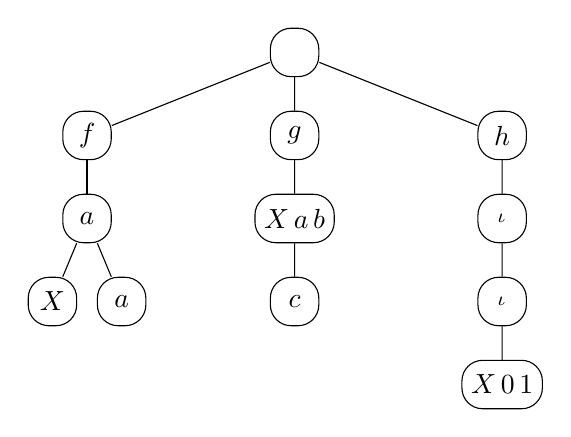
\begin{tikzpicture}[level distance=3em, sibling distance=7.5em,
  %  edge from parent path={(\tikzparentnode.south) -- ++(0,-0.5em)
  %   -| (\tikzchildnode.north)},
    every node/.style = {shape=rectangle, rounded corners=.75em, minimum size=1.75em, draw, align=center}]
    \node {\phantom{x}}
      child { node {$\cst{f}$}
        child[sibling distance=2.5em] { node %[fill=verylightgray]
          {$\cst{a}$}
          child {node {$X$}}
          child {node {$\cst{a}$}} }
      }
      child { node {$\cst{g}$}
        child {node {$X \, \cst{a} \, \cst{b}$}
               child {node {$\cst{c}$}}}
      }
      child { node {$\cst{h}$}
        child {node {$\internallam_\iota$}
          child {node {$\internallam_\iota$}
            child {node {$X \, \db{0} \, \db{1}$}}
          }
      }}
      ;
\end{tikzpicture}
\caption{First-order, $\lambda$-free higher-order, and higher-order pattern
  terms in a perfect discrimination tree}
\label{fig:pdt}
\end{figure}

In \ehohii{}, we extended this structure to support $\lambda$-abstractions and
the higher-order pattern matching algorithm.
To this end, we changed the way in which terms are
serialized. First, we require that all terms are fully $\eta$-expanded (except
for arguments of variables applied in patterns). Then, when the term is serialized,
we dedicate a separate node for applied variable terms $X \, \overline{s}_n$,
instead of the node for $X$ followed by nodes for serialization of arguments
$\overline{s}_n$. We serialize $\lambda$-abstraction $\lambda x.\, s$ using
a special node $\internallam_\tau$, where $\tau$ is the type of $x$,
followed by the serialization of $s$. Other than these two changes, serialization
remains as in Ehoh, following the gracefulness principle.
Figure \ref{fig:pdt} shows how $\cst{g} \,
(X\,\cst{a}\,\cst{b}) \, \cst{c}$ and $\cst{h} \, (\lambda x. \, \lambda y. \, X
\, y \, x)$ are serialized.

Since the terms are stored in serialized form, it is hard to manipulate
$\lambda$ prefixes of stored terms during matching. Performing $\eta$-expansion
when serializing terms makes sure that matchable terms have
$\lambda$ prefixes of the same length.

We have dedicated separate nodes for applied variables because access to arguments
of applied variables is necessary for the pattern matching algorithm. Even though
arguments can be obtained by querying the arity $n$ of the variable and taking
the next $n$ arguments in the serialization, this is both inefficient and inelegant.
As for De Bruijn indices, we treat them the same as function symbols and assign
them their own nodes.

\newcommand{\tstack}{\ensuremath{\texttt{term\_stack}}}
\newcommand{\tproc}{\ensuremath{\texttt{term\_proc}}}

\looseness=-1
Following the notation from the extension of perfect discrimination trees to
$\lambda$-free higher-order logic (Sect. \ref{sec:ehoh:indexing}), we now describe how enumeration of
generalizations is performed. To traverse the tree, \ehohii{} begins at the root
node and maintains two stacks:\ \tstack{} and \tproc{}, where \tstack{} contains the
subterms of the query term that have to be matched, and \tproc{} contains
processed terms that are used to backtrack to previous states. Initially,
\tstack{} contains the query term, the current matching substitution
$\sigma$ is empty, and the successor node is chosen among the child nodes as
follows:

\begin{enumerate}
\item[A.] If the node is labeled with a symbol $\xi$ (where
  $\xi$ is either a De Bruijn index or a constant) and the top item $t$
  of \tstack{} is of the form $\xi \, \overline{t}_n$, replace $t$ by
  $n$~new items $t_1,\dots,t_n$, and push $t$ onto \tproc{}.
\smallskip
\item[B.] If the node is labeled with a symbol $\internallam_\tau$ and the top
  item $t$ of \tstack{} is of the form $\lambda x.\, s$ and the type of $x$ is
  $\tau$, replace $t$ by $s$, and push $t$ onto \tproc{}.
\smallskip
\item[C.] If the node is labeled with a possibly applied variable $X \, \overline{s}_n$
  (where $n \geq 0$), and the top item of \tstack{} is $t$, the 
  matching algorithm described above is run on $X \, \overline{s}_n$ and $t$.
  The algorithm takes into account $\sigma$ built so far and extends it
  if necessary. If the algorithm succeeds, pop $t$ from \tstack{}, push it onto \tproc{},
  and save the original value of $\sigma$ in the node.
\end{enumerate}
  
Backtracking works in the opposite direction: If the current node is labeled with a De
Bruijn index or function symbol node of arity $n$, pop $n$ terms from \tstack{} and move the
top of \tproc{} to \tstack{}. If the node is labeled with
$\internallam_\tau$, pop the top of \tstack{} and move the top of \tproc{} to
\tstack{}. Finally, if the node is labeled with a possibly applied variable, move the top of the
\tproc{} to \tstack{} and restore the value of $\sigma$.

As an example of how finding a generalization works, consider the following
states of stacks and substitutions, which emerge when looking for generalizations of 
$\cst{g} \, (\cst{f} \, \cst{a} \, \cst{b}) \, \cst{c}$ in the tree of Figure \ref{fig:pdt}:
%
\[\begin{array}{@{}l@{\kern1em}l@{\kern1em}l@{\kern1em}l@{\kern1em}l@{}}
             & \epsilon                                                & \cst{g}                                                 & \cst{g}.(X \, \cst{a} \, \cst{b})                                                          & \cst{g}.(X \, \cst{a} \, \cst{b}).\cst{c} \\[.5\jot]
  \sigma{:}  & \emptyset                                               & \emptyset                                               & \{X \mapsto \cst{f}\}                                                                      & \{X \mapsto \cst{f}\} \\
  \tstack{:} & [\cst{g} \, (\cst{f} \, \cst{a} \, \cst{b}) \, \cst{c}] & [\cst{f} \, \cst{a} \, \cst{b}, \cst{c}]                & [\cst{c}]                                                                                  & [] \\
  \tproc{:}  & []                                                      & [\cst{g} \, (\cst{f} \, \cst{a} \, \cst{b}) \, \cst{c}] & [\cst{f} \, \cst{a} \, \cst{b}{,}\; \cst{g} \, (\cst{f} \, \cst{a} \, \cst{b}) \, \cst{c}] & [\cst{c}{,}\;\cst{f} \, \cst{a} \, \cst{b}{,}\; \cst{g} \, (\cst{f} \, \cst{a} \, \cst{b}) \, \cst{c}]
  \end{array}\]

  \section{Preprocessing, Calculus, and Extensions}
  \label{sec:ehoh2:calculus}
  
  Ehoh's simple $\lambda$-free higher-order calculus performed well on
  Sledgehammer problems and formed a promising stepping stone to full higher-order
  logic (Sect.~\ref{sec:ehoh:evaluation}). When implementing support for full higher-order
  logic, we were guided by efficiency and gracefulness with respect to Ehoh's calculus rather
  than completeness. Whereas Zipperposition provides both complete and incomplete
  modes, \ehohii{} only offers incomplete modes.
  
  \ourpara{Preprocessing} Our experience with Zipperposition showed the importance
  of flexibility in preprocessing the higher-order problems
  (Sect.~\ref{sec:ho-tech:preprocessing}). Therefore, we implemented a flexible
  preprocessing module in \ehohii{}. 
  
  To maintain compatibility with Ehoh, \ehohii{} can optionally transform all
  $\lambda$-abstractions into named functions. This process is called
  \emph{$\lambda$-lifting} \cite{rjmh-82-lifting}. \ehohii{} also removes all
  occurrences of Boolean subterms (other than $\itrue, \ifalse$, and free variables)
  in higher-order contexts using a FOOL-like transformation \cite{kotelnikov-16-fool}.
  For example, the formula $\cst{f}(\cst{p} \iand \cst{q}) \ieq \cst{a}$ becomes
  $(\cst{p} \iand \cst{q} \iimplies \cst{f}(\itrue) \ieq \cst{a}) \iand
  (\inot(\cst{p} \iand \cst{q}) \iimplies \cst{f}(\ifalse) \ieq \cst{a})$.
  
  \looseness=-1
  Many TPTP problems use the \texttt{definition} role to denote the definitions of
  symbols. \ehohii{} can treat the definition axioms as rewrite rules, and replace
  all occurrences of defined symbols during preprocessing. Furthermore, during
  SInE \cite{hv-2011-sine} axiom selection, it can always
  include the defined symbol in the trigger relation.
  
  \ourpara{Calculus} \ehohii{} implements the same superposition
  calculus as Ehoh with three important changes. First, wherever Ehoh requires
  the MGU of terms, \ehohii{} enumerates unifiers from a finite subset of the CSU, as explained in
  Sect.~\ref{sec:ehoh2:unif-match-index}. Second, \ehohii{} uses versions of the KBO and
  LPO orders designed for $\lambda$-terms.
  % as described by Bentkamp et al.\ \cite{bbtv-21-full-ho-sup}.
  
  %TODO: @JASMIN: How do we cite the STTT article?
  The third difference is more subtle. One of the main features of Ehoh is
  \emph{prefix optimization} (Sect.~\ref{sec:ehoh:introduction}): a method that, given a demodulator $s \eq t$, allows
  to replace both applied and unapplied occurrences of $s$ by $t$ 
  by traversing only first-order subterms of a rewritable term. In a $\lambda$-free setting this
  optimization is useful, but in the presence of $\beta\eta$-normalization, shapes of
  terms can change drastically, making it much harder to
  track prefixes of terms. This is why we disabled the prefix optimization in \ehohii{}.
  To counterbalance this removal, we introduced
  the argument congruence rule \infname{AC} %(also called \infname{ArgCong})
  in \ehohii{}
  and enabled positive and negative functional extensionality (\infname{PE} and
  \infname{NE}) by default:
  
  \vskip\abovedisplayskip
  
  \noindent\hbox{}\hfill
    \namedinference{AC}{s \eq t \llor C}{s \, X \eq t \, X \llor C}%
  \hfill
    \namedinference{NE}{s \noteq t \llor C}{s \; (\cst{sk} \; \overline{X}) \noteq t \; (\cst{sk} \; \overline{X}) \llor C}%
  \hfill
    \namedinference{PE}{s \; X \eq t \; X \llor C}{s \eq t \llor C}%
  \hfill\hbox{}
  
  \vskip\belowdisplayskip
  
  \noindent
  \infname{AC} and \infname{NE} assume that $s$ and $t$ are of function
  type. In \infname{NE}, $\overline{X}$ denotes all the free variables occurring in $s$ and
  $t$, and $\cst{sk}$ is a fresh Skolem symbol of the appropriate type. \infname{PE}
  has a side condition that $X$ may not appear in $s$, $t$, or $C$.
  
  \ourpara{Saturation} E's saturation procedure is based on the assumption that
  each attempt to perform an inference will either result in a single clause or
  fail due to one of the inference side conditions. Unification procedures that
  produce multiple substitutions break this invariant, and the saturation
  procedure needed to be adjusted.
  
  In Sect.~\ref{sec:ho-tech:infinite-branching}, we described a variant of the saturation
  procedure that elegantly supports interleaving computations of unifiers and
  scheduling
  inferences to be performed. Since completeness was
  not one of the \ehohii{} design goals, we did not implement this version of the
  saturation procedure. Instead, in places where previously a single unifier was
  expected, \ehohii{} consumes all elements of the iterator used for enumerating a
  unifier, converting them to clauses. 
  
  \ourpara{Reasoning about Formulas} Even though most of the Boolean structure is
  removed during preprocessing, formulas can reappear at the top level of
  clauses during saturation. For example, after replacing $X$ with $\lambda x.
  \, \lambda y.\, x \iand y$, the clause $X \, \cst{p} \, \cst{q} \llor \cst{a}
  \eq \cst{b}$ becomes $(\cst{p} \iand \cst{q}) \llor \cst{a} \eq \cst{b}$. \ehohii{}
  converts every clause of the form $\varphi \llor C$, where $\varphi$ has a logic symbol
  as its head (or it is a (dis)equation between two formulas different than $\itrue$),
  to an explicitly quantified formula. Then, the clausification algorithm
  is invoked on the formula to restore the clausal structure. Zipperposition features
  more dynamic clausification modes, but for simplicity we decided
  not to implement them in \ehohii{}.
  
  The \osup{} calculus
  \cite{bbtv-21-full-ho-sup} includes many rules that act on Boolean subterms,
  which are necessary for completeness. Other than Boolean simplification rules,
  which use simple tautologies such as $\cst{p} \iand \itrue \iequiv\cst{p}$ to simplify terms, we
  have implemented none of the Boolean rules of this calculus in \ehohii{}. First, we have
  observed that complicated rules such as \infname{FluidBoolHoist} and
  \infname{FluidLoobHoist} are hardly ever useful in practice and usually only
  contribute to an uncontrolled increase in the proof state size. Second, simpler
  rules such as \infname{BoolHoist} can usually be simulated by pragmatic rules
  that perform Boolean and functional extensionality reasoning, described below.
  
  To make up for excluding Boolean rules, we use an incomplete, but more
  easily controllable and intuitive rule, called \emph{primitive instantiation}. This
  rule instantiates free predicate variables with approximations of formulas
  that are ground instances of this variable. We described this rule in Sect.~\ref{sect:bool:native}.
  In \ehohii{} it is implemented in a similar manner.
  
  \ehohii{}'s handling of the Hilbert choice operator is inspired by Leo-III's
  \cite{sb-21-leo3}. \ehohii{}
  recognizes clauses of the form $\neg P \, X \lor P \, (\cst{f} \, P)$ which
  essentially denote that $\cst{f}$ is a choice symbol. Then, when subterm
  $\cst{f} \, s$ is found during saturation, $s$ is used to instantiate the choice
  axiom for $\cst{f}$. 
  %
  Similarly, Leibniz equality is eliminated by
  recognizing clauses of the form  $\neg P \, \cst{a} \llor P \, \cst{b} \llor C$. These clauses are then
  instantiated with $P \mapsto \lambda x. \, x \eq \cst{a}$ and $P \mapsto \lambda
  x. \, x\noteq\cst{b}$, which results in $\cst{a} \eq \cst{b} \lor C$. Both rules
  are described in Sect.~\ref{sect:bool:native} in more detail.
  
  Finally, \ehohii{} treats induction axioms specially. Just like
  Zipperposition (Sect.~\ref{sec:ho-tech:formulas}), it abstracts literals
  from the goal clauses and uses these abstractions to instantiate induction
  axioms. Since Zipperposition supports dynamic calculus-level clausification,
  instantiation of induction axioms happens during saturation, when these axioms
  are processed. In \ehohii{}, this instantiation is performed statically,
  immediately after clausification. After \ehohii{} collects all the abstractions,
  it traverses the clauses and instantiates those that have applied variable of
  the same type as the abstraction.
  
  \begin{sloppypar}
    \ourpara{Extensionality} \ehohii{} takes a pragmatic approach to reasoning about
    functional and Boolean extensionality: It uses \emph{abstracting} rules (\infname{Abs} rules of Sect.~\ref{sect:bool:native}) 
    which simulate basic superposition calculus rules,
    but do not require unifiability of the partner terms in the inference. More
    precisely, assume a core inference needs to be performed between two
    $\beta$-reduced terms $u$ and $v$, such that they can be represented as
    $u=C[s_1, \ldots, s_n]$ and $v=C[t_1, \ldots, t_n]$, where $C$ is the most general
    common context (more precisely, green common context that does not go into the structure of $\lambda$-abstraction or applied variables \cite{bbtvw-21-sup-lam}) of $u$ and $v$, not all of
    $s_i$ and $t_j$ are free variables, and for at least one $i$, $s_i \not= t_i$,
    $s_i$ and $t_i$ are not (possibly applied) free variables, and they are of Boolean or
    function type. Then, the conclusion is formed by taking the conclusion $D$ of
    the core inference rule (which would be created if $s$ and $t$ are unifiable)
    and adding literals $s_1 \noteq t_1 \llor \cdots \llor s_n \noteq t_n$.
      
  \end{sloppypar}
  
  These rules are particularly useful because \ehohii{} has no rules that dynamically
  process Booleans in FOOL-like fashion, such as \infname{BoolHoist}. For example,
  given the clauses $\cst{f} \, (\cst{p} \iand \cst{q})\allowbreak \eq \cst{a}$ and
  $\cst{g} \, (\cst{f} \, \cst{p}) \noteq \cst{b}$, the abstracting version of the
  superposition rules \infname{SP} and \infname{SN} (Sect.~\ref{sec:pre:rules}) would result in $\cst{g} \, \cst{a} \noteq \cst{b} \llor (\cst{p}
  \iand \cst{q}) \noteq \cst{p}$. In this way, the Boolean structure bubbles up to
  the top level and is further processed by clausification. We noticed that this
  alleviates the need for the other Boolean rules in practice.

  \section{Evaluation}
  \label{sec:ehoh2:eval}
  
  In this section, we try to answer two questions about \ehohii{}: \emph{How does
  \ehohii{} compare against other higher-order provers (including Ehoh)?} \emph{Does
  \ehohii{} introduce any overhead compared with Ehoh?} To answer
  these questions, we ran provers on problems from the TPTP library \cite{gs-17-tptp} and on
  benchmarks generated by Sledgehammer (SH) \cite{pb-12-sh}.
  The experiments were carried out on StarExec Miami
  \cite{sst-14-starexec} nodes equipped with Intel Xeon E5-2620 v4 CPU clocked at
  2.10~GHz. For the TPTP part, we used the CASC-28\footnote{\url{http://www.tptp.org/CASC/28/}} time limits:\ 120~s
  wall-clock and 960~s CPU. For SH benchmarks and to answer the other question, we used Sledgehammer's
  default time limit:\ 30~s wall-clock and CPU.  The raw evaluation data is available online\footnote{\url{https://doi.org/10.5281/zenodo.6389849}}.

  
  \ourpara{Comparison with Other Provers}
  To answer the first question, we let
  \ehohii{} compete with the top contenders in the higher-order division of
  CASC-28:\ cvc5 \NumberOK{0.0.7},\footnote{\url{https://cvc5.github.io/}}
  Ehoh 2.7, Leo-III \NumberOK{1.6.6} \cite{sb-21-leo3}, Vampire 4.6
  \cite{br-20-full-sup-w-combs}, and Zipperposition 2.1 (Chapter~\ref{ch:ho-techniques}). 
  We also included Satallax 3.5
  \cite{cb-12-satallax}. We used all \NumberOK{2899} higher-order
  theorems in TPTP 7.5.0 as well as 5000 SH higher-order benchmarks
  originating from the Seventeen benchmark suite \cite{desharnais-et-al-202x}.
  On SH benchmarks,
  cvc5, Ehoh, \ehohii{}, Vampire, and Zipperposition were run using custom schedules provided by
  their developers, optimized for single-core usage and low timeouts.
  Otherwise, we used the corresponding CASC configurations.
  Note that Ehoh 2.7 is an updated version of Ehoh described in Chapter
  \ref{ch:ehoh}, which can parse not only $\lambda$-free but also full
  higher-order. It is only a syntactic extension as $\lambda$-abstractions are supported using $\lambda$-lifting \cite{rjmh-82-lifting}.
  We included two versions of Zipperposition:\ \emph{coop} uses Ehoh 2.7 as a backend to finish proof attempts,
  whereas \emph{uncoop} does not use this feature. The results
  are shown in Figure \ref{fig:all-provers}.
  
  Both Ehoh and \ehohii{} were run in the automatic scheduling mode. Compared to Ehoh,
  \ehohii{} features a redesigned module for automatic scheduling, it
  can use multiple CPU cores, and its heuristics have been trained better on higher-order problems.
  
  \ehohii{} dramatically improves the higher-order reasoning capabilities
  compared to Ehoh. It solves \NumberOK{20\%} more problems on TPTP benchmarks
  and \NumberOK{6\%} more problems on SH benchmarks, where Ehoh was already very
  successful.
  
  \ehohii{} was mainly designed as an efficient backend to proof assistants. As such it 
  excels on SH benchmarks, outperforming the competition. On TPTP, it outperforms all higher-order provers other than Zipperposition-coop.
  If Zipperposition's Ehoh backend is disabled,
  \ehohii{} outperforms Zipperposition by a wide margin.
  This comparison is arguably fairer; after all,
  \ehohii{} does not use an older version of Zipperposition
  as a backend.
  %
  These results suggest that \ehohii{} already implements most of the necessary features
  for a high-performance higher-order prover
  but could benefit from the kind of fine-tuning that
  Zipperposition underwent in the last two years.
  
  Remarkably, there is a substantial disparity in the set of problems solved by
  \ehohii{} and Zipperposition-coop. The raw data show thats \ehohii{} solves
  \NumberOK{166} SH problems and \NumberOK{21} TPTP problems that Zipperposition-coop
  does not. The lower number of uniquely solved TPTP problems is most likely 
  due to Zipperposition's being heavily optimized on TPTP.
  
  \ourpara{Comparison with the First-Order E} Both Ehoh and \ehohii{} can be compiled
  in a mode that disables most of the higher-order reasoning. This mode is
  designed for users that are interested only in E's first-order capabilities and
  care a lot about performance.
  To answer the second
  evaluation question, about assessing overhead of \ehohii{},
  we chose all the \NumberOK{1138} unique problems used at CASC
  from 2019 to 2021 in the first-order theorem division and ran Ehoh and \ehohii{}
  both in this first-order (FO) mode and in higher-order (HO) mode.
  
  We fixed a single
  configuration of options, because Ehoh's and \ehohii{}'s
  automatic scheduling methods could select different configurations
  and we would not be measuring the overhead but the quality of the chosen
  configurations. We chose the \emph{boa} configuration (Sect.~\ref{sec:ehoh:heuristics}),
  which is the configuration that E~2.2 used most often in its automatic scheduling mode.
  The results are shown in Figure~\ref{fig:ehoh}.
  
  Counterintuitively, the higher-order versions of both provers outperform
  the first-order counterparts. However, the difference is so small that it can
  be attributed to the changes to memory layout that affect the order in which
  clauses are chosen. Similar effects are seen when comparing the first-order versions.
  We would expected the less heavily modified version of E, Ehoh, to perform better,
  but due to subtle effects \ehohii{} wins.
  
  
  \begin{figure}[t]
    \noindent\hbox{}\hfill
    \begin{minipage}[ht!]{.66\linewidth}
      \centering
      \def\arraystretch{1.1}%
      \relax{\begin{tabular}{l@{\hskip 1em}@{\hskip 0.5em}c@{\hskip 1em}c} \toprule
               
                              & TPTP       & SH        \\
        \midrule
        cvc5                  & 1931       & 2577      \\
        Ehoh                  & 2105       & 2611      \\
        \ehohii{}             & 2523       & {\bf 2766}\\
        Leo-III               & 2282       & 1601      \\
        Satallax              & 2320       & 1719      \\
        Vampire               & 2203       & 2240      \\
        Zipperposition-coop   & {\bf 2583} & 2754      \\
        Zipperposition-uncoop & 2483       & 2181      \\
        \bottomrule
      \end{tabular}}
      \caption{Comparison of higher-order provers}
      \label{fig:all-provers}
    \end{minipage}\hfill\hfill
    \begin{minipage}[ht!]{.30\linewidth}
      \centering
      \def\arraystretch{1.1}%
      \relax{\begin{tabular}{l@{\hskip 1em}@{\hskip 0.5em}c} \toprule
                        & TPTP     \\
        \midrule
        Ehoh FO      & 535      \\
        Ehoh HO      & 538      \\
        \ehohii{} FO & {\bf 539}\\
        \ehohii{} HO & {\bf 539}\\
        \bottomrule
      \end{tabular}}
      \caption{Evaluation of \ehohii{}'s overhead}
      \label{fig:ehoh}
    \end{minipage}\hfill\hfill
  \end{figure}
  

  \section{Discussion and Related Work} %---0.5p
  \label{sec:ehoh2:discussion}
  
  \looseness=-1
  On the trajectory to \ehohii{}, we developed, together with colleagues, three
  superposition calculi:\ \lfsup{} for $\lambda$-free higher-order logic
  \cite{bbcw-21-lfho}, \lsup{} for a higher-order logic with
  $\lambda$-abstra\-ction but no Booleans \cite{bbtvw-21-sup-lam}, and \osup{}
  for full higher-order logic \cite{bbtvw-21-sup-lam}. These milestones allowed
  us to carefully estimate how the increased reasoning capabilities of each
  calculus influence its performance. We also developed a complete and efficient
  unification algorithm (Chapter \ref{ch:unif}) which can easily be customized
  to trade bits of its completeness for efficiency. Practically oriented work,
  described in Chapters \ref{ch:bools} and \ref{ch:ho-techniques},
  helped us gauge how much reasoning power we lose by using more intuitive and
  more easily controllable incomplete rules. Both the theoretical and the
  practical lines of our work met in this chapter, resulting in a prover that
  outperforms the competition on the benchmarks from proof assistants.
  
  Extending first-order provers with higher-order reasoning capabilities has been
  attempted by other researchers as well.
  Barbosa et al.\ extended
  the SMT solvers CVC4 (now cvc5) and veriT to higher-order logic in an incomplete
  way \cite{brotb-19-ho-smt}.
  Bhayat and Reger first extended Vampire to
  higher-order logic using combinatory unification \cite{br-19-restricted-unif},
  an incomplete approach, before they designed and implemented a complete
  higher-order superposition calculus based on \textsf{SKBCI}-com\-binators \cite{br-20-full-sup-w-combs}.
  The advantage is that combinators can be supported as a thin layer on top of
  $\lambda$-free terms.
  This calculus is also implemented in Zipperposition.
  However, in informal experiments, we found that $\lambda$-superposition
  performs substantially better, corroborating the CASC results, so we decided to
  make a more profound change to Ehoh and implement $\lambda$-superposition.
  \pagebreak[2]

  Possibly the only actively maintained higher-order prover built from the bottom
  up as a higher-order prover is Leo-III \cite{sb-21-leo3}, as the long-time
  winner of CASC higher-order division, Satallax \cite{cb-12-satallax}, is no
  longer maintained. A further overview of other traditional higher-order provers and the calculi they are based on can be found in Sect.~\ref{sec:ehoh:discussion-and-related-work}.
  
  \section{Conclusion} %---0.5p
  \label{sec:ehoh2:conclusion}
  
  In 2019, the reviewers of our paper introducing Ehoh \cite{vbss-19-ehoh1} were
  skeptical that extending it with support for full higher-order logic would be
  feasible. One of them wrote:
  %
  \begin{quote}
  A potential criticism could be that this step from E to Ehoh is just extending
  FOL by those aspects of HOL that are easily in reach with rather straightforward
  extensions (none of the extensions is indeed very complicated), and that the
  difficult challenges of fully supporting HOL have yet to be confronted.
  \end{quote}
  %
  We ended up addressing the theoretical ``difficult challenges'' in other work
  with colleagues. In this chapter, we faced the practical challenges pertaining to the extension
  of Ehoh's data structures and algorithms to support full higher-order logic and
  demonstrated that such an extension is possible. \NumberOK{Our evaluation} shows
  that this extension makes \ehohii{} the best higher-order prover on
  benchmarks coming from interactive theorem proving practice, which was our goal. \ehohii{}
  lags slightly behind Zipperposition on TPTP problems, possibly because Zipperposition
  does not assume a clausal structure and can perform subtle formula-level
  inferences. In the future, we plan to implement the same features in \ehohii{}.
  We have also only started tuning \ehohii{}'s heuristics on higher-order
  problems.
